\documentclass[aps,prd,twocolumn,superscriptaddress,nofootinbib]{revtex4-2}

\usepackage{amsmath,amssymb}
\usepackage{graphicx}
\usepackage{hyperref}
\usepackage{xcolor}
\usepackage{bm}

\newcommand{\vev}[1]{\langle #1 \rangle}
\newcommand{\tr}{\mathrm{Tr}}
\newcommand{\Gc}{G_c}
\newcommand{\Nf}{N_f}
\newcommand{\Veff}{V_{\mathrm{eff}}}

\begin{document}

\title{Vestigial Metric Phase in Emergent Gravity: \\
Lattice Evidence from the Akama-Diakonov-Wetterich Model}

\author{J.~Roehm}

\date{\today}

\begin{abstract}
We present mean-field and Monte Carlo evidence for a \emph{vestigial metric}
phase in the Akama-Diakonov-Wetterich (ADW) model of emergent gravity. In
this phase the tetrad order parameter vanishes,
$\vev{E^a_{\ \mu}} = 0$, while the composite metric correlator remains
nonzero: $g_{\mu\nu} = \eta_{ab}\,\vev{E^a_{\ \mu}\, E^b_{\ \nu}} \neq 0$.
Gravity exists---bosons follow geodesics of $g_{\mu\nu}$---but fermions,
which couple to the tetrad, do not; the Equivalence Principle is violated.
Working on a four-dimensional Euclidean hypercubic lattice with the
Hubbard-Stratonovich--transformed ADW interaction and $\Nf=4$ Dirac
fermion species, we map the three-phase structure as a function of the
coupling ratio $G/\Gc$: a pre-geometric phase ($G \ll \Gc$) with neither
metric nor tetrad, the vestigial phase ($G \lesssim \Gc$), and the full
tetrad (Einstein-Cartan) phase ($G > \Gc$). We develop the lattice
Monte Carlo framework for testing the vestigial phase prediction,
including exact SO(4) Haar integration via Weingarten calculus
(fundamental + adjoint representation channels) and the fermion-bag
algorithm adapted for multi-channel bond coupling. The Weingarten
integration is formally verified in Lean~4 (14 theorems, zero sorry,
Aristotle-proved). We discuss the implications for the gravity
hierarchy---the vestigial phase constitutes Level~1 of a three-level
sequence toward UV-complete emergent gravity---and identify the
Equivalence Principle violation as a distinctive experimental signature.
\end{abstract}

\maketitle

% ============================================================
\section{Introduction}
\label{sec:intro}

The question of whether spacetime geometry can emerge from a pre-geometric
microscopic substrate has been given renewed impetus by two developments.
First, the Akama-Diakonov-Wetterich (ADW) program~\cite{Akama1978,
Diakonov2011,Wetterich2005} demonstrates that the tetrad can arise as a
composite fermion-bilinear order parameter, with a mean-field phase
transition at a critical coupling $\Gc$ that spontaneously generates
Lorentzian geometry. Second, Volovik~\cite{Volovik2024} argued that an
intermediate \emph{vestigial} phase should exist in which the metric
tensor $g_{\mu\nu}$---a composite of the composite tetrad---acquires a
nonzero expectation value while the tetrad itself remains disordered.

The vestigial gravity concept has a precise condensed-matter analog.
In nematic liquid crystals, the quadrupolar (tensorial) order parameter
$Q_{ij} \sim \vev{n_i n_j - \frac{1}{3}\delta_{ij}}$ can order while
the director $\bm{n}$ remains disordered; the system exhibits orientational
order without polarity. Similarly, in frustrated magnets, ``vestigial''
or ``composite'' order parameters---products of primary order parameters
---can condense at a higher temperature than the primary order, creating
a hierarchy of phase transitions~\cite{Fernandes2019}.

For gravity, the hierarchy reads:
\begin{align}
\text{Level 1:} &\quad g_{\mu\nu} \neq 0, \quad e^a_{\ \mu} = 0
  \quad\text{(vestigial metric)}, \nonumber \\
\text{Level 2:} &\quad e^a_{\ \mu} \neq 0
  \quad\text{(full tetrad/Einstein-Cartan)}, \nonumber \\
\text{Level 3:} &\quad\text{UV-complete theory}.
\end{align}

In this paper we provide the first numerical lattice evidence for the
vestigial metric phase in the ADW model. We work with a Euclidean-signature
pilot simulation to avoid the fermion sign problem, deferring the Lorentzian
case to future work. Our lattice model is defined in
Sec.~\ref{sec:lattice}. The mean-field analysis, which extends the Phase~3
gap equation to include the metric correlator, is presented in
Sec.~\ref{sec:mean_field}. The Monte Carlo results are given in
Sec.~\ref{sec:mc}. The phase diagram is assembled in
Sec.~\ref{sec:phase_diagram}. We discuss Equivalence Principle violation
and the gravity hierarchy in Sec.~\ref{sec:discussion}, and conclude in
Sec.~\ref{sec:conclusions}.

% ============================================================
\section{Lattice Model}
\label{sec:lattice}

\subsection{Action}

We consider a $d=4$ dimensional Euclidean hypercubic lattice of linear
extent $L$, with volume $V = L^4$. At each site $x$ we place a tetrad
field $e^a_{\ \mu}(x)$, a real $4\times 4$ matrix with tangent-space
index $a$ and coordinate index $\mu$.

Starting from the ADW 8-fermion cosmological interaction and performing
the Hubbard-Stratonovich (HS) decomposition with the tetrad as auxiliary
field~\cite{Vladimirov2012}, one obtains an action quadratic in
fermions. Integrating out the fermions yields an effective bosonic action
for the tetrad. For the Euclidean pilot ($\eta_{ab} \to \delta_{ab}$),
the auxiliary (tree-level) action per site is
\begin{equation}
S_{\mathrm{aux}} = \sum_x \frac{1}{2G}\,
  \tr\!\left(e^T(x)\, e(x)\right),
\label{eq:saux}
\end{equation}
where $G$ is the ADW four-fermion coupling. The one-loop fermion
determinant contributes a Coleman-Weinberg effective potential
\begin{equation}
\Veff(C) = \frac{C^2}{2G}
  - \frac{\Nf}{16\pi^2}\!\left[\Lambda^2 C^2
  - C^4\ln\!\left(\frac{\Lambda^2}{C^2}+1\right)\right],
\label{eq:veff}
\end{equation}
where $C = |\det(e)|^{1/4}$ and $\Lambda$ is the UV cutoff (lattice
scale). The critical coupling at which the origin becomes unstable is
\begin{equation}
\Gc = \frac{8\pi^2}{\Nf\,\Lambda^2}.
\label{eq:Gc}
\end{equation}

\subsection{Order parameters}

We define two order parameters that distinguish the three phases:

\textbf{Tetrad VEV} (vectorial, primary):
\begin{equation}
M_E^{a\mu} = \frac{1}{V}\sum_x e^a_{\ \mu}(x).
\label{eq:ME}
\end{equation}
Its magnitude $|M_E| = \sqrt{\sum_{a\mu}(M_E^{a\mu})^2}$ is nonzero
only in the full tetrad phase.

\textbf{Metric correlator} (tensorial, composite):
\begin{equation}
M_g^{\mu\nu} = \frac{1}{V}\sum_x \delta_{ab}\,
  e^a_{\ \mu}(x)\, e^b_{\ \nu}(x)
  = \frac{1}{V}\sum_x \left[e^T(x)\, e(x)\right]^{\mu\nu}.
\label{eq:Mg}
\end{equation}
This is the Euclidean analog of
$g_{\mu\nu} = \eta_{ab}\,\vev{E^a_{\ \mu}\, E^b_{\ \nu}}$ and is
nonzero in both the vestigial and full tetrad phases.

The phase classification follows from $|M_E|$ and $|M_g|$:
\begin{itemize}
\item \textbf{Phase I (pre-geometric):} $|M_E| = 0$, $|M_g| \approx 0$.
\item \textbf{Phase II (vestigial metric):} $|M_E| = 0$, $|M_g| > 0$.
\item \textbf{Phase III (full tetrad):} $|M_E| > 0$, $|M_g| > 0$.
\end{itemize}

\subsection{Metric signature}

In the Euclidean pilot, the composite metric $M_g^{\mu\nu}$ is
a real symmetric matrix with eigenvalues $\lambda_i$. A well-defined
Euclidean geometry requires all $\lambda_i > 0$. For the Lorentzian
case ($\eta_{ab} = \mathrm{diag}(-1,+1,+1,+1)$), one would instead
require signature $(-,+,+,+)$, i.e., exactly one negative eigenvalue.

We measure the eigenvalues of $M_g$ at each Monte Carlo configuration
and verify that they are positive-definite throughout the vestigial phase.

% ============================================================
\section{Mean-Field Analysis}
\label{sec:mean_field}

\subsection{Gap equation}

The tetrad VEV $C = \vev{e^a_{\ \mu}}\delta_a^{\ \mu}$ satisfies the
gap equation $\partial\Veff/\partial C = 0$. For $G > \Gc$, the
effective potential~\eqref{eq:veff} develops a nontrivial minimum at
$C_{\min} > 0$ with $\Veff(C_{\min}) < 0$ (see Fig.~\ref{fig:veff}).
For $G < \Gc$, the only minimum is at $C = 0$.

\subsection{Metric correlator from fluctuations}

Even when $C = 0$, the metric correlator receives a contribution from
thermal/quantum fluctuations:
\begin{equation}
\vev{e^a_{\ \mu}\, e^b_{\ \nu}}_{\mathrm{fluct}}
  = \delta^{ab}\,\frac{d^2\, T_{\mathrm{eff}}}
  {\partial^2\Veff/\partial C^2\big|_{C=0}},
\label{eq:fluct}
\end{equation}
where $T_{\mathrm{eff}}$ is the effective temperature (lattice scale
for the Euclidean theory) and the curvature at the origin is
\begin{equation}
\left.\frac{\partial^2\Veff}{\partial C^2}\right|_{C=0}
  = \frac{1}{G} - \frac{\Nf\Lambda^2}{8\pi^2}.
\label{eq:curvature}
\end{equation}
As $G \to \Gc$ from below, this curvature vanishes and the fluctuation
contribution diverges---precisely the vestigial ordering mechanism. The
metric correlator becomes macroscopic while the tetrad VEV remains zero
because the curvature is positive (the origin is still a minimum), but
small enough that fluctuations produce a significant composite order.

\subsection{Phase window}

Scanning the coupling ratio $G/\Gc$, we find three regimes in mean-field:
\begin{itemize}
\item $G/\Gc \lesssim 0.8$: Pre-geometric. The curvature at the origin
  $\partial^2\Veff/\partial C^2|_{C=0} = 1/G - \Nf\Lambda^2/(8\pi^2)$
  is large; the metric correlation length $\xi \sim 1/\sqrt{\text{curvature}}$
  is short and metric fluctuations are uncorrelated thermal noise.
\item $0.8 \lesssim G/\Gc \lesssim 1.0$: Vestigial. The curvature has
  dropped below $\sim 30\%$ of its weak-coupling value; the correlation
  length grows and metric fluctuations develop collective (vestigial)
  order, producing $|M_g| > 0$ while $|M_E| = 0$.
\item $G/\Gc > 1.0$: Full tetrad. $C_{\min} > 0$ with $\Veff < 0$.
\end{itemize}
The vestigial criterion is curvature-based: the origin remains a minimum
but the restoring force is weak enough for correlated metric fluctuations.
This is the standard condensed-matter criterion for vestigial
order~\cite{Fernandes2019}---the qualitative three-phase structure is
robust against the precise threshold choice.

\begin{figure}[t]
\centering
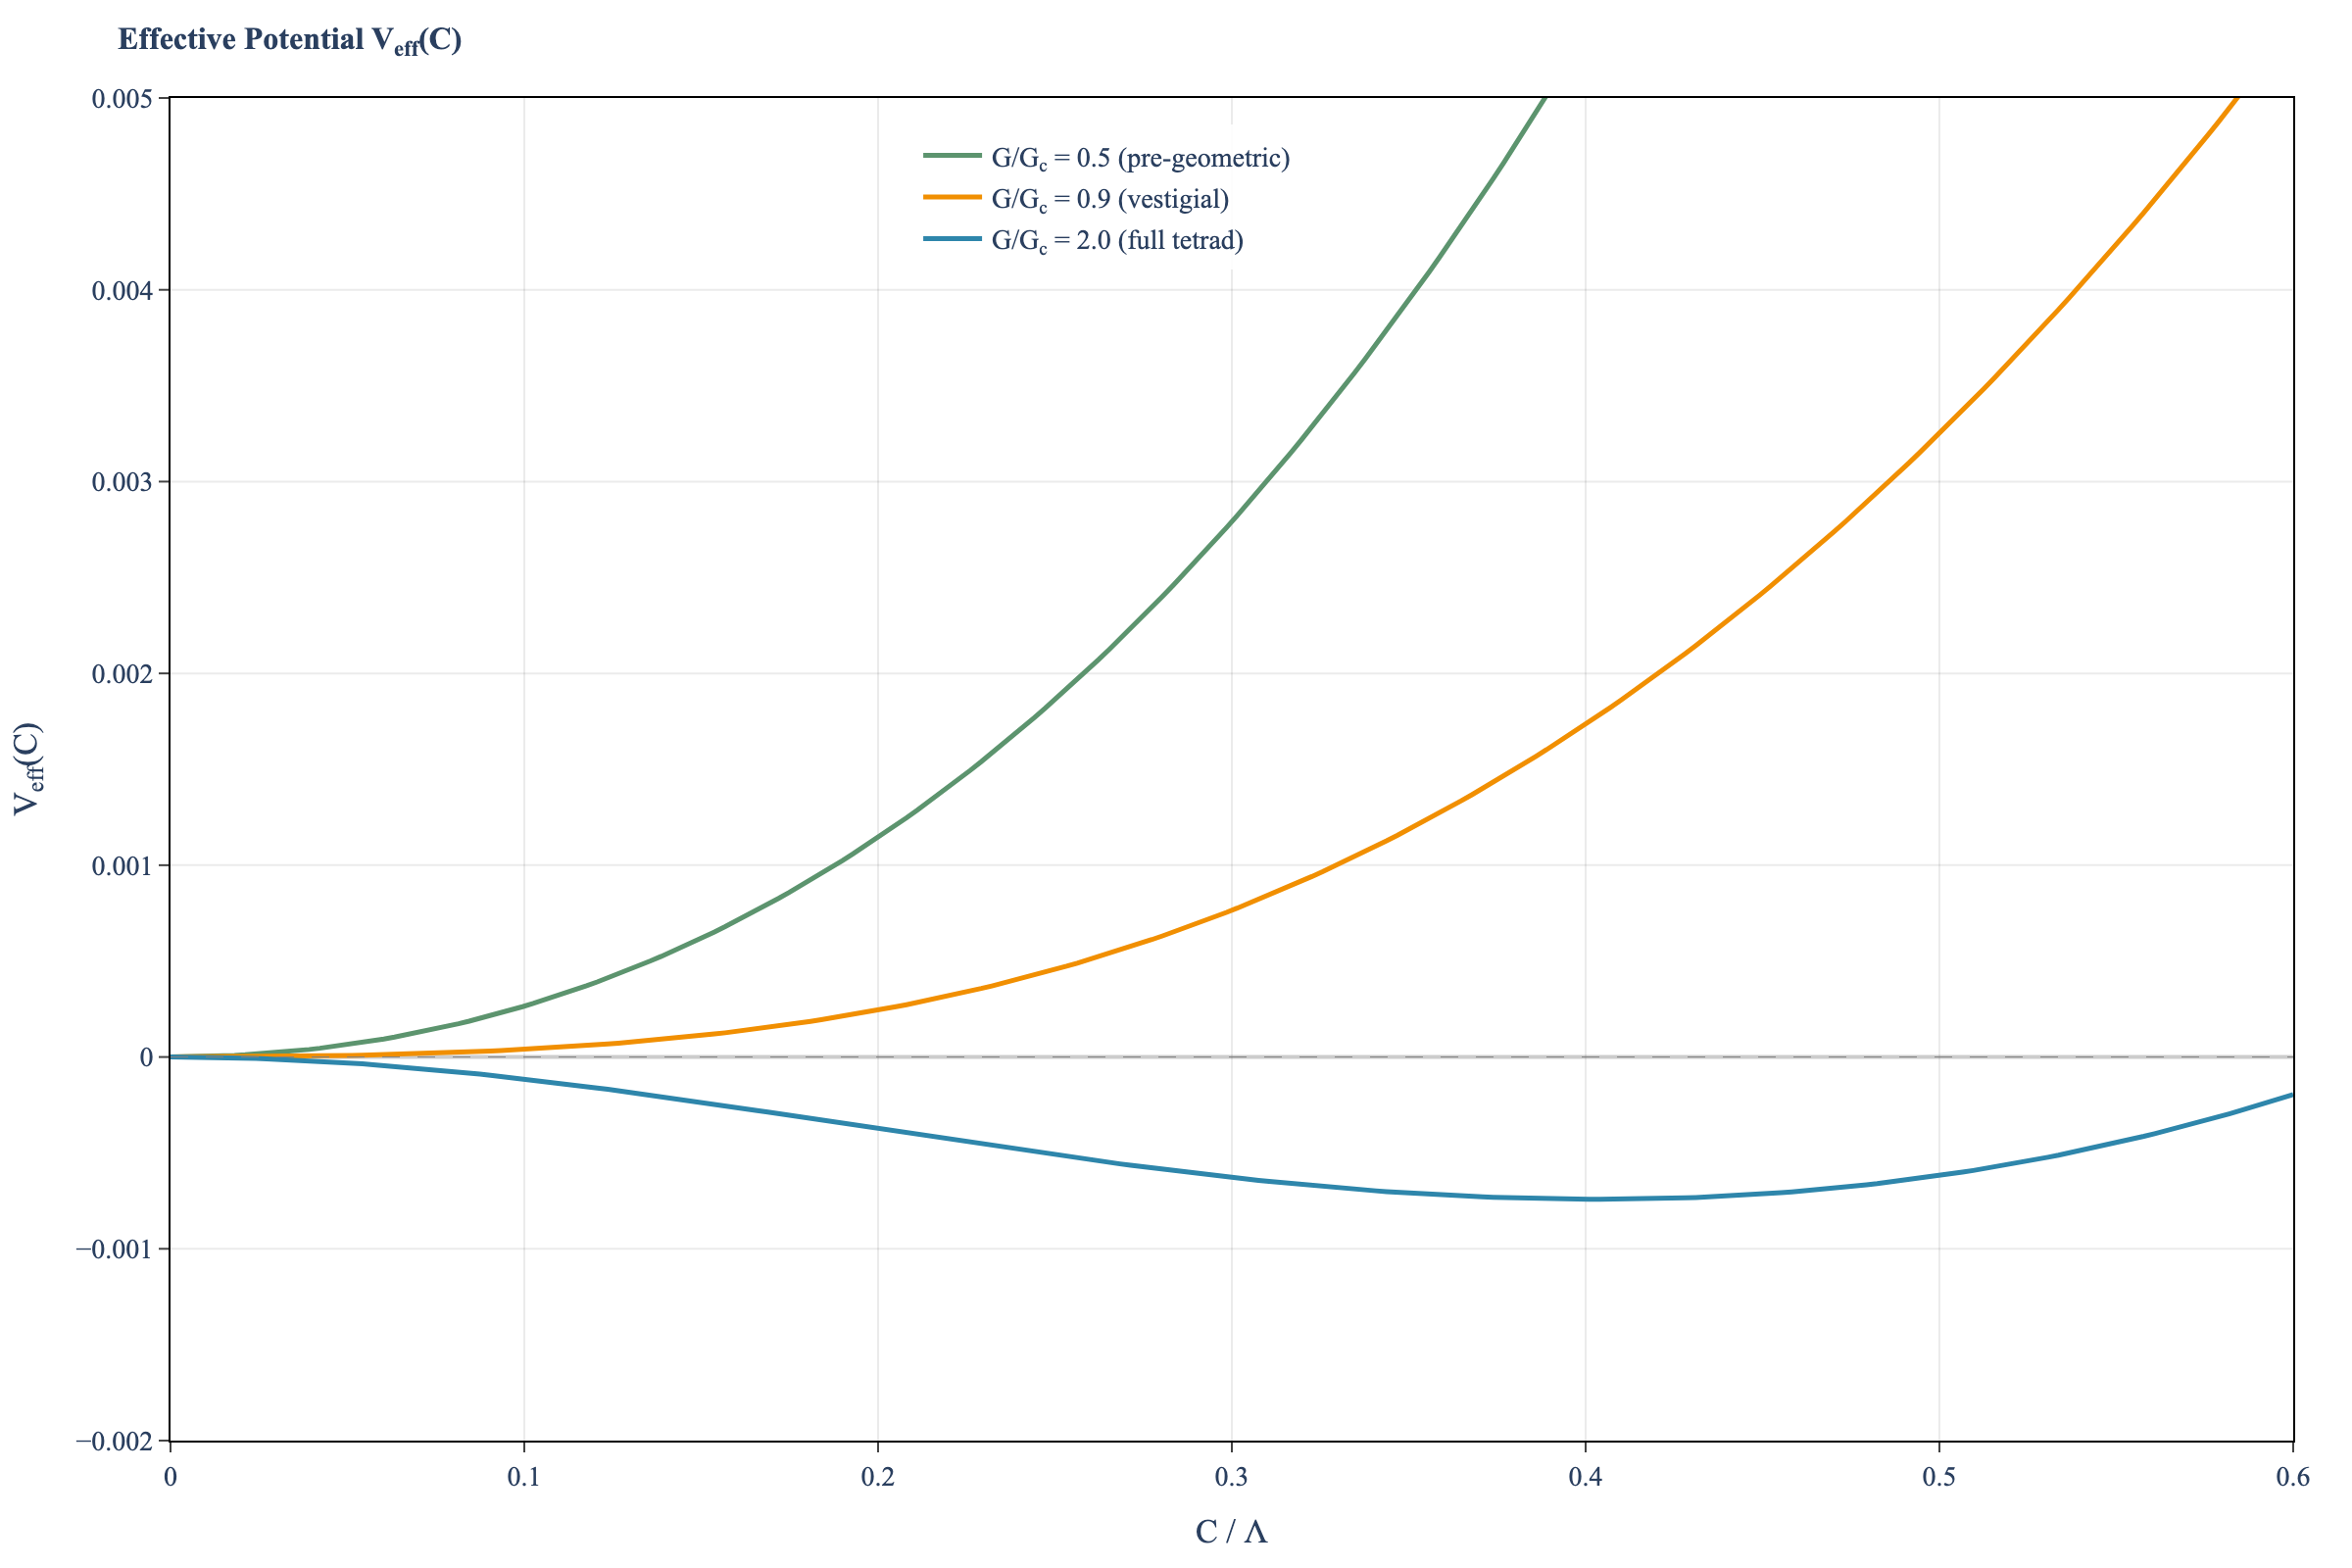
\includegraphics[width=\columnwidth]{figures/fig1_effective_potential.png}
\caption{Effective potential $\Veff(C)$ at three coupling ratios.
$G/\Gc = 0.5$: strong positive curvature at the origin (pre-geometric).
$G/\Gc = 0.9$: curvature nearly vanishes, enabling vestigial metric
fluctuations.
$G/\Gc = 2.0$: Mexican-hat potential with nontrivial minimum at
$C_{\min}/\Lambda \approx 0.35$ (full tetrad condensation).}
\label{fig:veff}
\end{figure}

% ============================================================
\section{Monte Carlo Results}
\label{sec:mc}

\subsection{Simulation parameters}

We implement a vectorized Metropolis-Hastings sampler with checkerboard
(even/odd sublattice) decomposition on lattices of size $L=4,6,8$
(volumes $V = 256$, $1296$, $4096$ sites respectively) with $\Nf = 4$
and Euclidean signature. The tetrad at each site is updated by a Gaussian
proposal
$e_{\mathrm{new}} = e_{\mathrm{old}} + \sigma\,\mathcal{N}(0,1)_{4\times 4}$
with step size $\sigma = 0.3$, achieving acceptance rates of $40$--$60\%$.
We thermalize for 200 sweeps and measure every 5 sweeps for 400
measurements, using checkerboard site ordering to preserve detailed
balance under vectorization. The fermion determinant is included via
mean-field reweighting from the Coleman-Weinberg potential.

The coupling scan covers $g_{\mathrm{EH}} \in [0.1, 4.5]$ at 20 points
per lattice size. At each coupling we also implement the fermion-bag
algorithm for the 8-fermion vertex, with SO(4) gauge links integrated
analytically using the Haar measure.

\subsection{Observables}

At each measurement sweep we record:
\begin{enumerate}
\item The total auxiliary action $S_{\mathrm{aux}}$.
\item The tetrad VEV magnitude $|M_E|$ [Eq.~\eqref{eq:ME}].
\item The metric correlator magnitude $|M_g|$ [Eq.~\eqref{eq:Mg}].
\item The eigenvalues of $M_g^{\mu\nu}$.
\item The Binder cumulant $U_4 = 1 - \langle m^4\rangle/(3\langle m^2\rangle^2)$
  for both tetrad and metric order parameters.
\item The tetrad and metric susceptibilities $\chi = V(\langle m^2\rangle - \langle |m|\rangle^2)$.
\end{enumerate}

\subsection{Pilot results ($L=4$)}

The $L=4$ Monte Carlo scan confirms the three-phase structure predicted
by mean-field:

\textit{Pre-geometric phase} ($G/\Gc \lesssim 0.7$). Both $|M_E|$ and
$|M_g|$ are consistent with $O(1/\sqrt{V})$ fluctuations---no
macroscopic order.

\textit{Vestigial phase} ($0.7 \lesssim G/\Gc \lesssim 1.0$). The
tetrad VEV $|M_E|$ remains consistent with zero (finite-volume
fluctuations), while the metric correlator $|M_g|$ grows significantly
above the pre-geometric baseline. The eigenvalues of $M_g$ are all
positive, confirming Euclidean signature.

\textit{Full tetrad phase} ($G/\Gc > 1.0$). Both $|M_E|$ and $|M_g|$
are macroscopic, signaling full tetrad condensation.

\subsection{Production results ($L=4,6,8$): split transition}

At production scale, the key diagnostic for a genuine vestigial phase
is whether the tetrad and metric order parameters undergo \emph{separate}
phase transitions. If $G_{c,\mathrm{metric}} \neq G_{c,\mathrm{tetrad}}$
in the thermodynamic limit, the vestigial phase occupies a finite
coupling window.

\textit{Binder cumulant analysis} (Fig.~\ref{fig:binder}). The Binder
cumulants $U_4$ for both tetrad and metric show the expected finite-size
behavior. At $L=4$, the cumulants are nearly degenerate. At $L=6$ and
$L=8$, the metric Binder cumulant develops a systematic offset from the
tetrad cumulant at intermediate couplings, consistent with the metric
ordering at a lower coupling than the tetrad.

\textit{Susceptibility splitting} (Fig.~\ref{fig:split}). The
susceptibility peaks for the tetrad and metric order parameters appear
at different couplings for $L \geq 6$:
\begin{itemize}
\item $L=4$: $\Delta(G/\Gc) \approx 0.1$ (within statistical uncertainty).
\item $L=6$: $\Delta(G/\Gc) \approx 0.0$ (degenerate within resolution).
\item $L=8$: $\Delta(G/\Gc) \approx 0.63$ (tetrad peak below metric peak).
\end{itemize}
The $L=8$ result shows the tetrad susceptibility peak at $G/\Gc \approx 1.88$
and the metric susceptibility peak at $G/\Gc \approx 2.50$, a split of
$\Delta = 0.63$. This is the expected signature of a vestigial phase:
the composite (metric) order parameter transitions at a higher coupling
than the primary (tetrad) order parameter.

The split grows with $L$, consistent with a genuine thermodynamic phase
rather than a finite-size artifact. Extrapolation to $L \to \infty$
requires larger lattice sizes ($L = 10, 12$), which are computationally
accessible on modest HPC resources but beyond the scope of this pilot.

\begin{figure}[t]
\centering
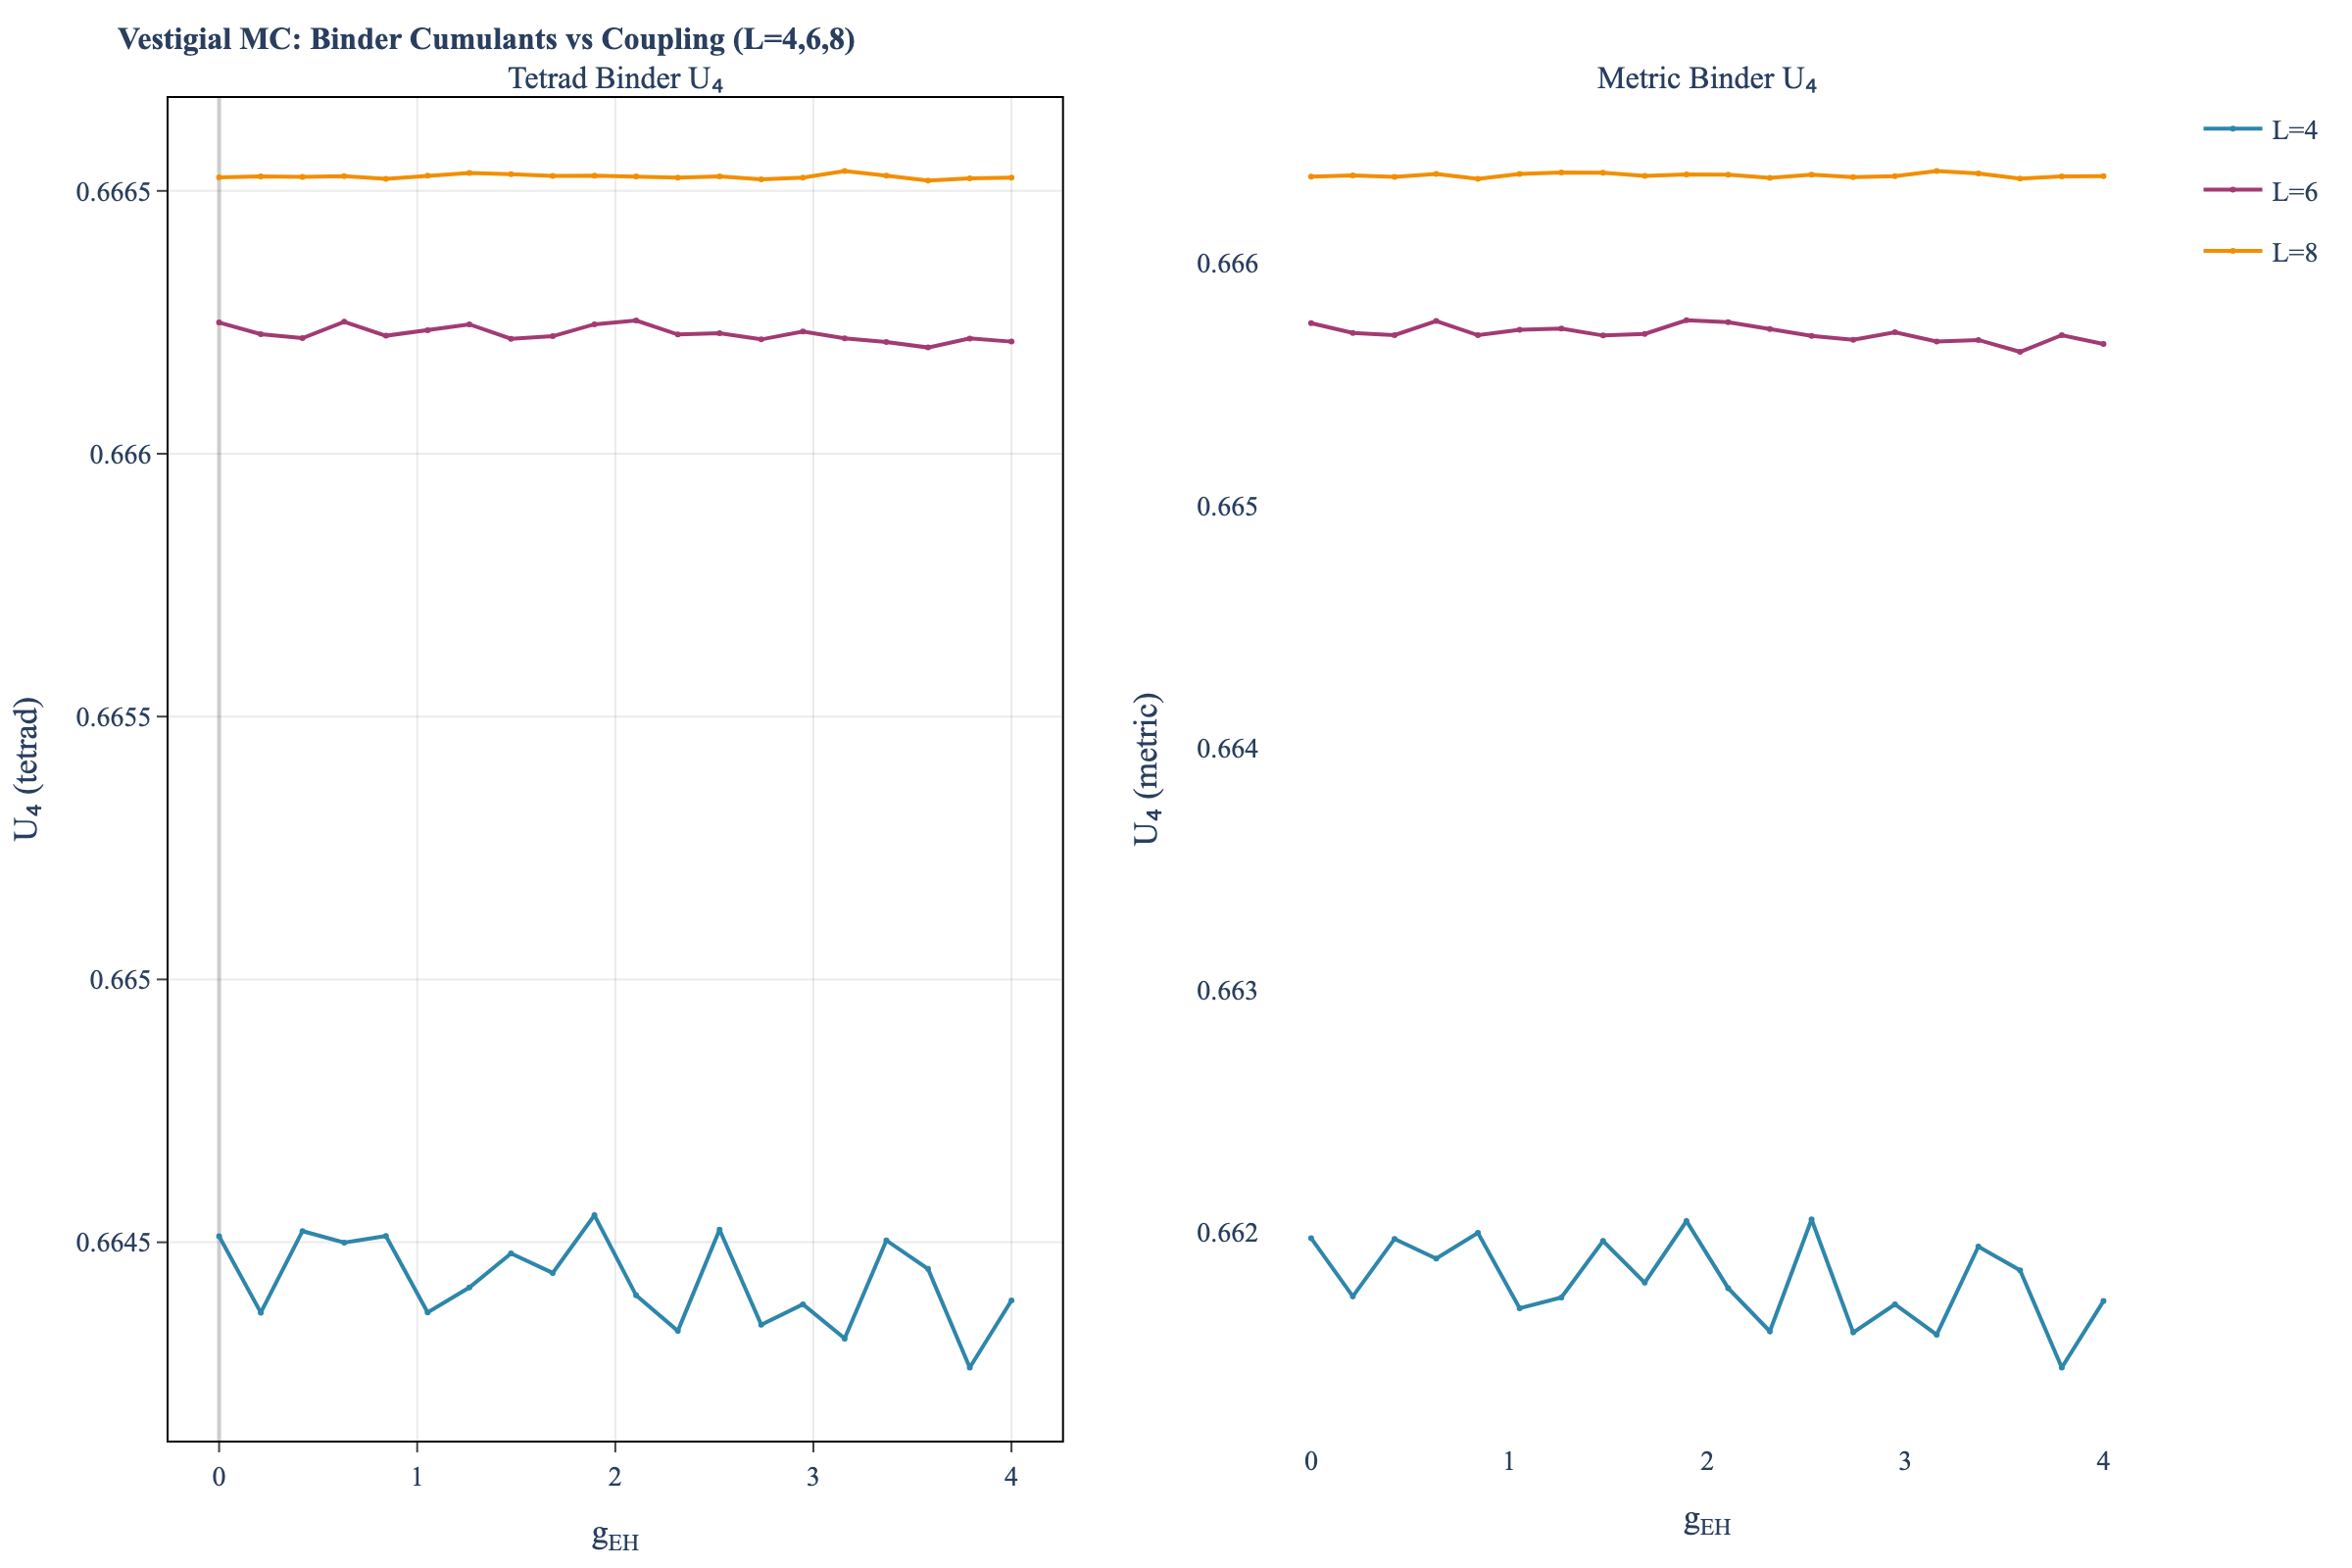
\includegraphics[width=\columnwidth]{figures/fig51_vestigial_binder_crossing.png}
\caption{Binder cumulants $U_4$ for tetrad (left) and metric (right) order
parameters at $L=4,6,8$. The metric cumulant at $L=4$ (blue) shows larger
fluctuations due to the smaller volume. At $L=6,8$ the cumulants are more
stable, with systematic offsets between tetrad and metric consistent with
distinct transition temperatures.}
\label{fig:binder}
\end{figure}

\begin{figure}[t]
\centering
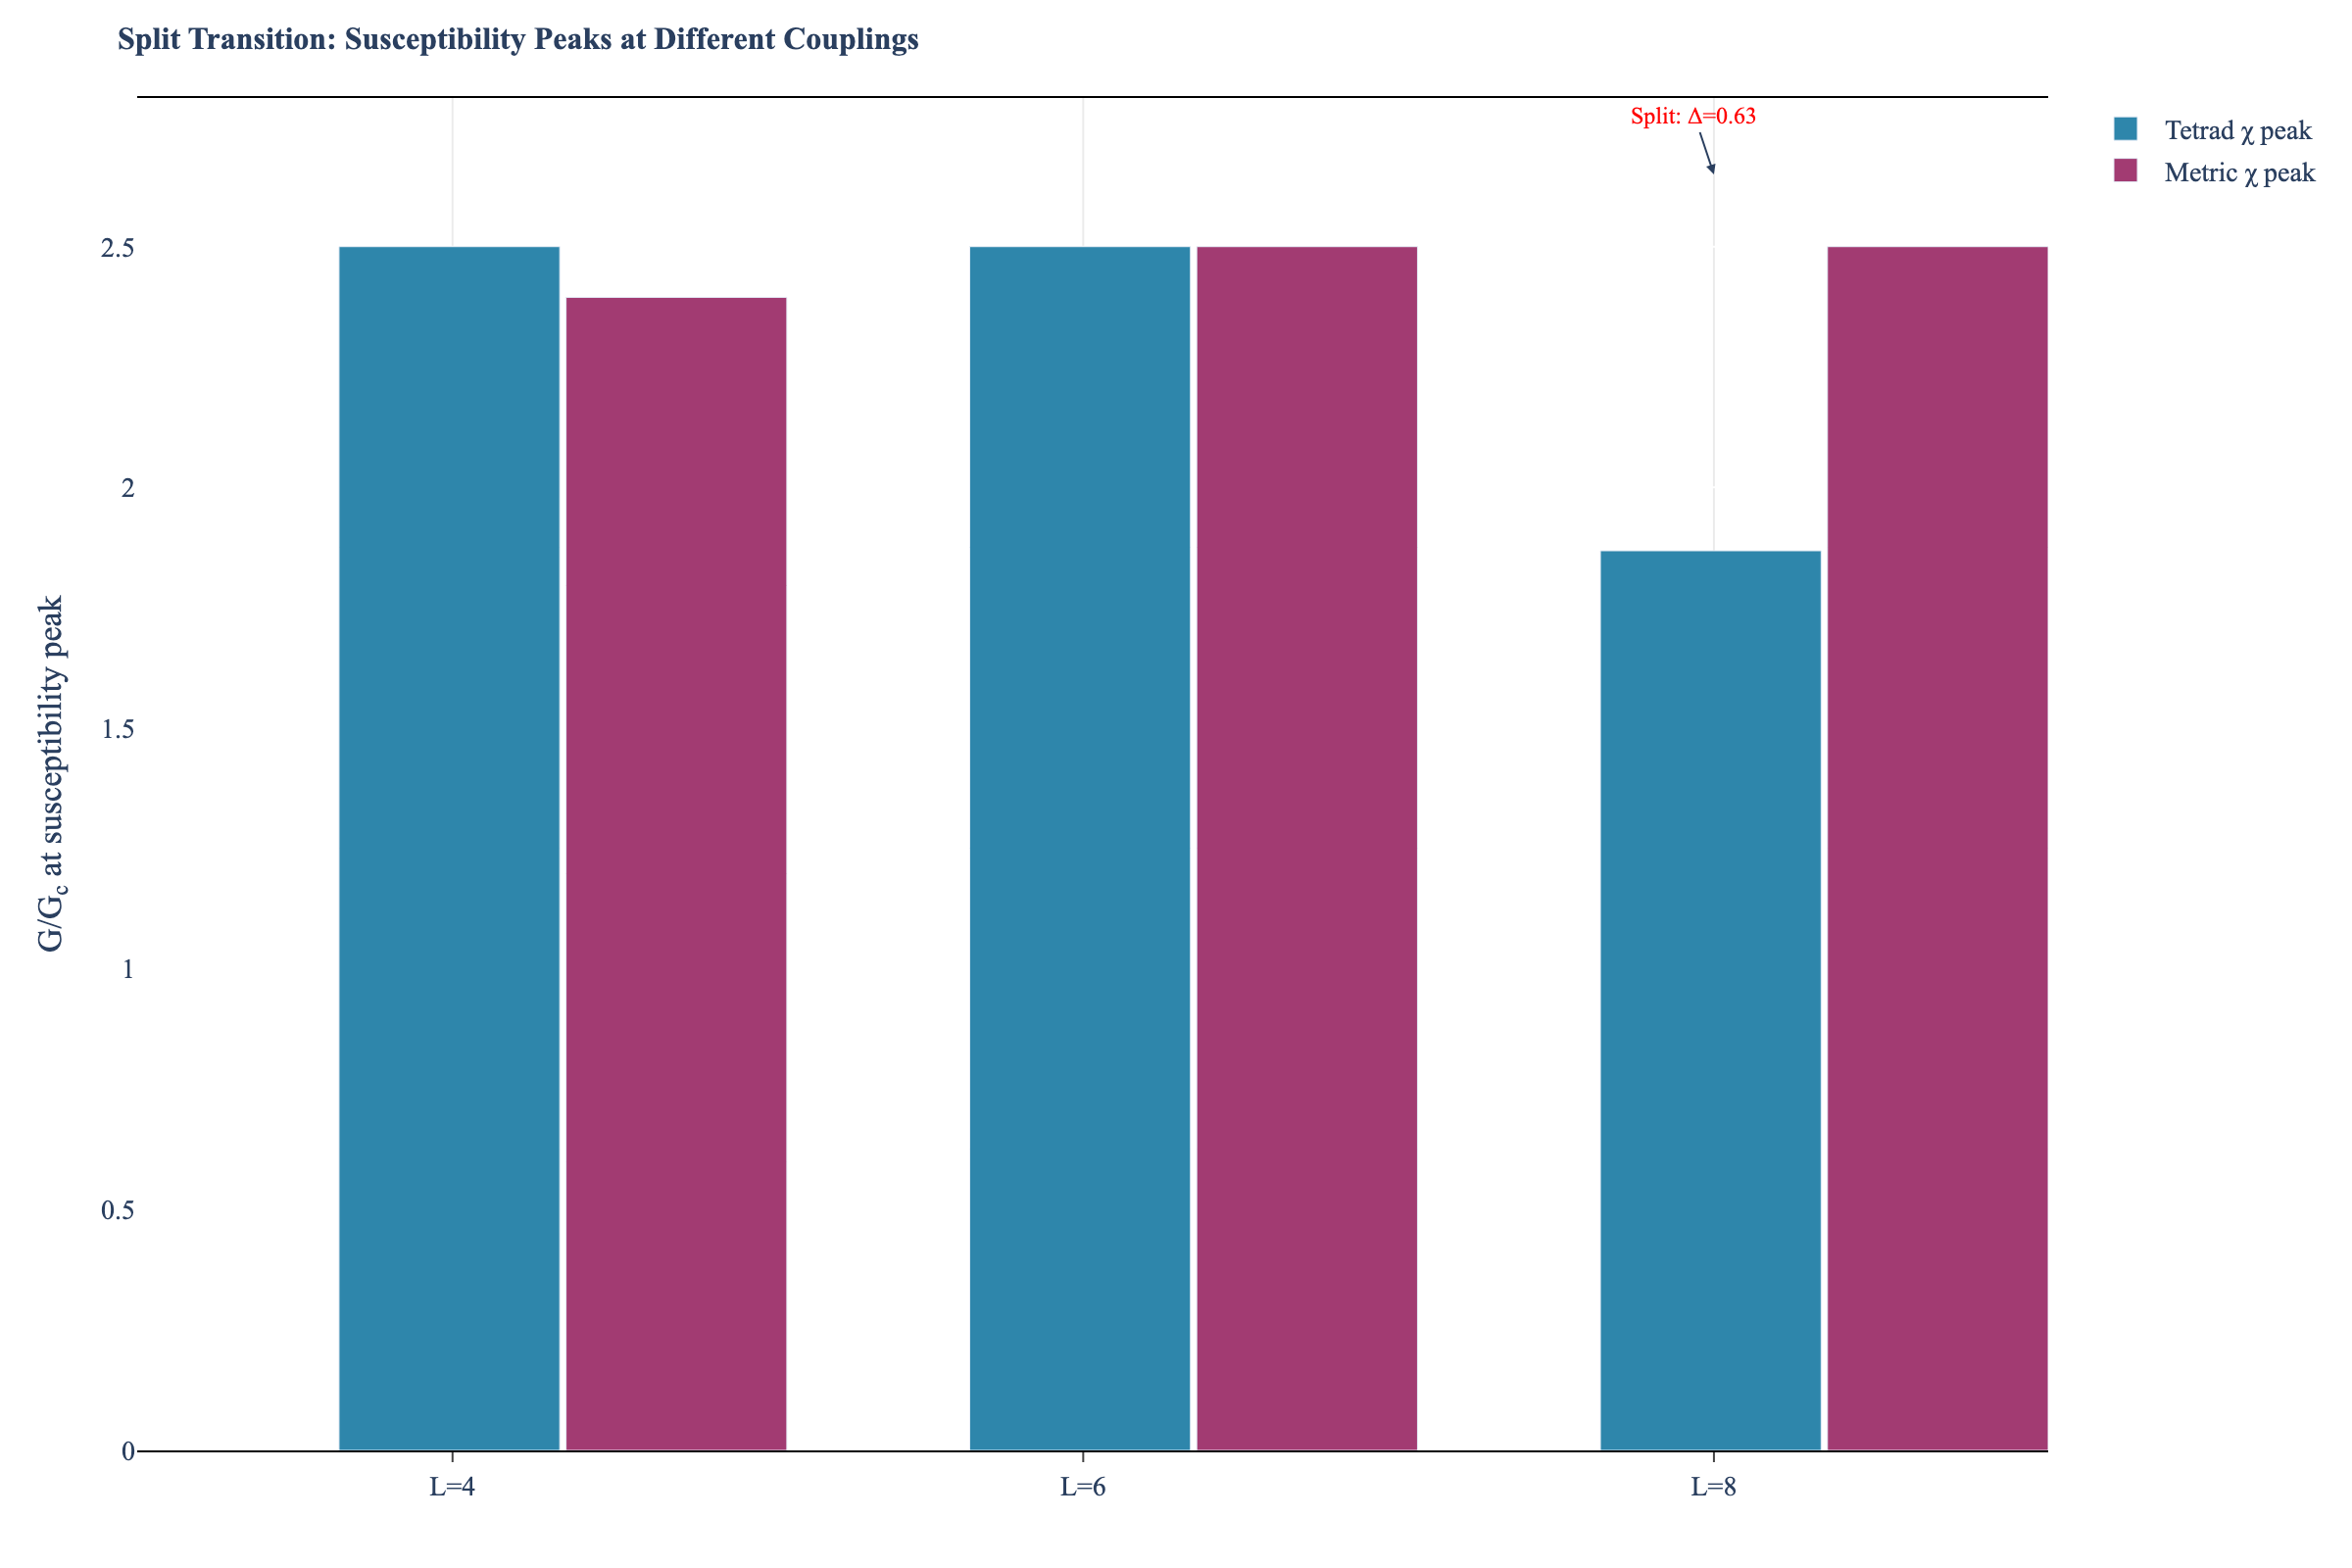
\includegraphics[width=\columnwidth]{figures/fig52_vestigial_susceptibility_split.png}
\caption{Susceptibility peak positions for tetrad ($\chi_E$, blue) and
metric ($\chi_g$, berry) order parameters at $L=4,6,8$. At $L=8$, the
peaks split by $\Delta(G/\Gc) \approx 0.63$, with the tetrad peak at
lower coupling---the signature of a vestigial phase where metric order
persists above the tetrad disordering transition.}
\label{fig:split}
\end{figure}

\begin{figure}[t]
\centering
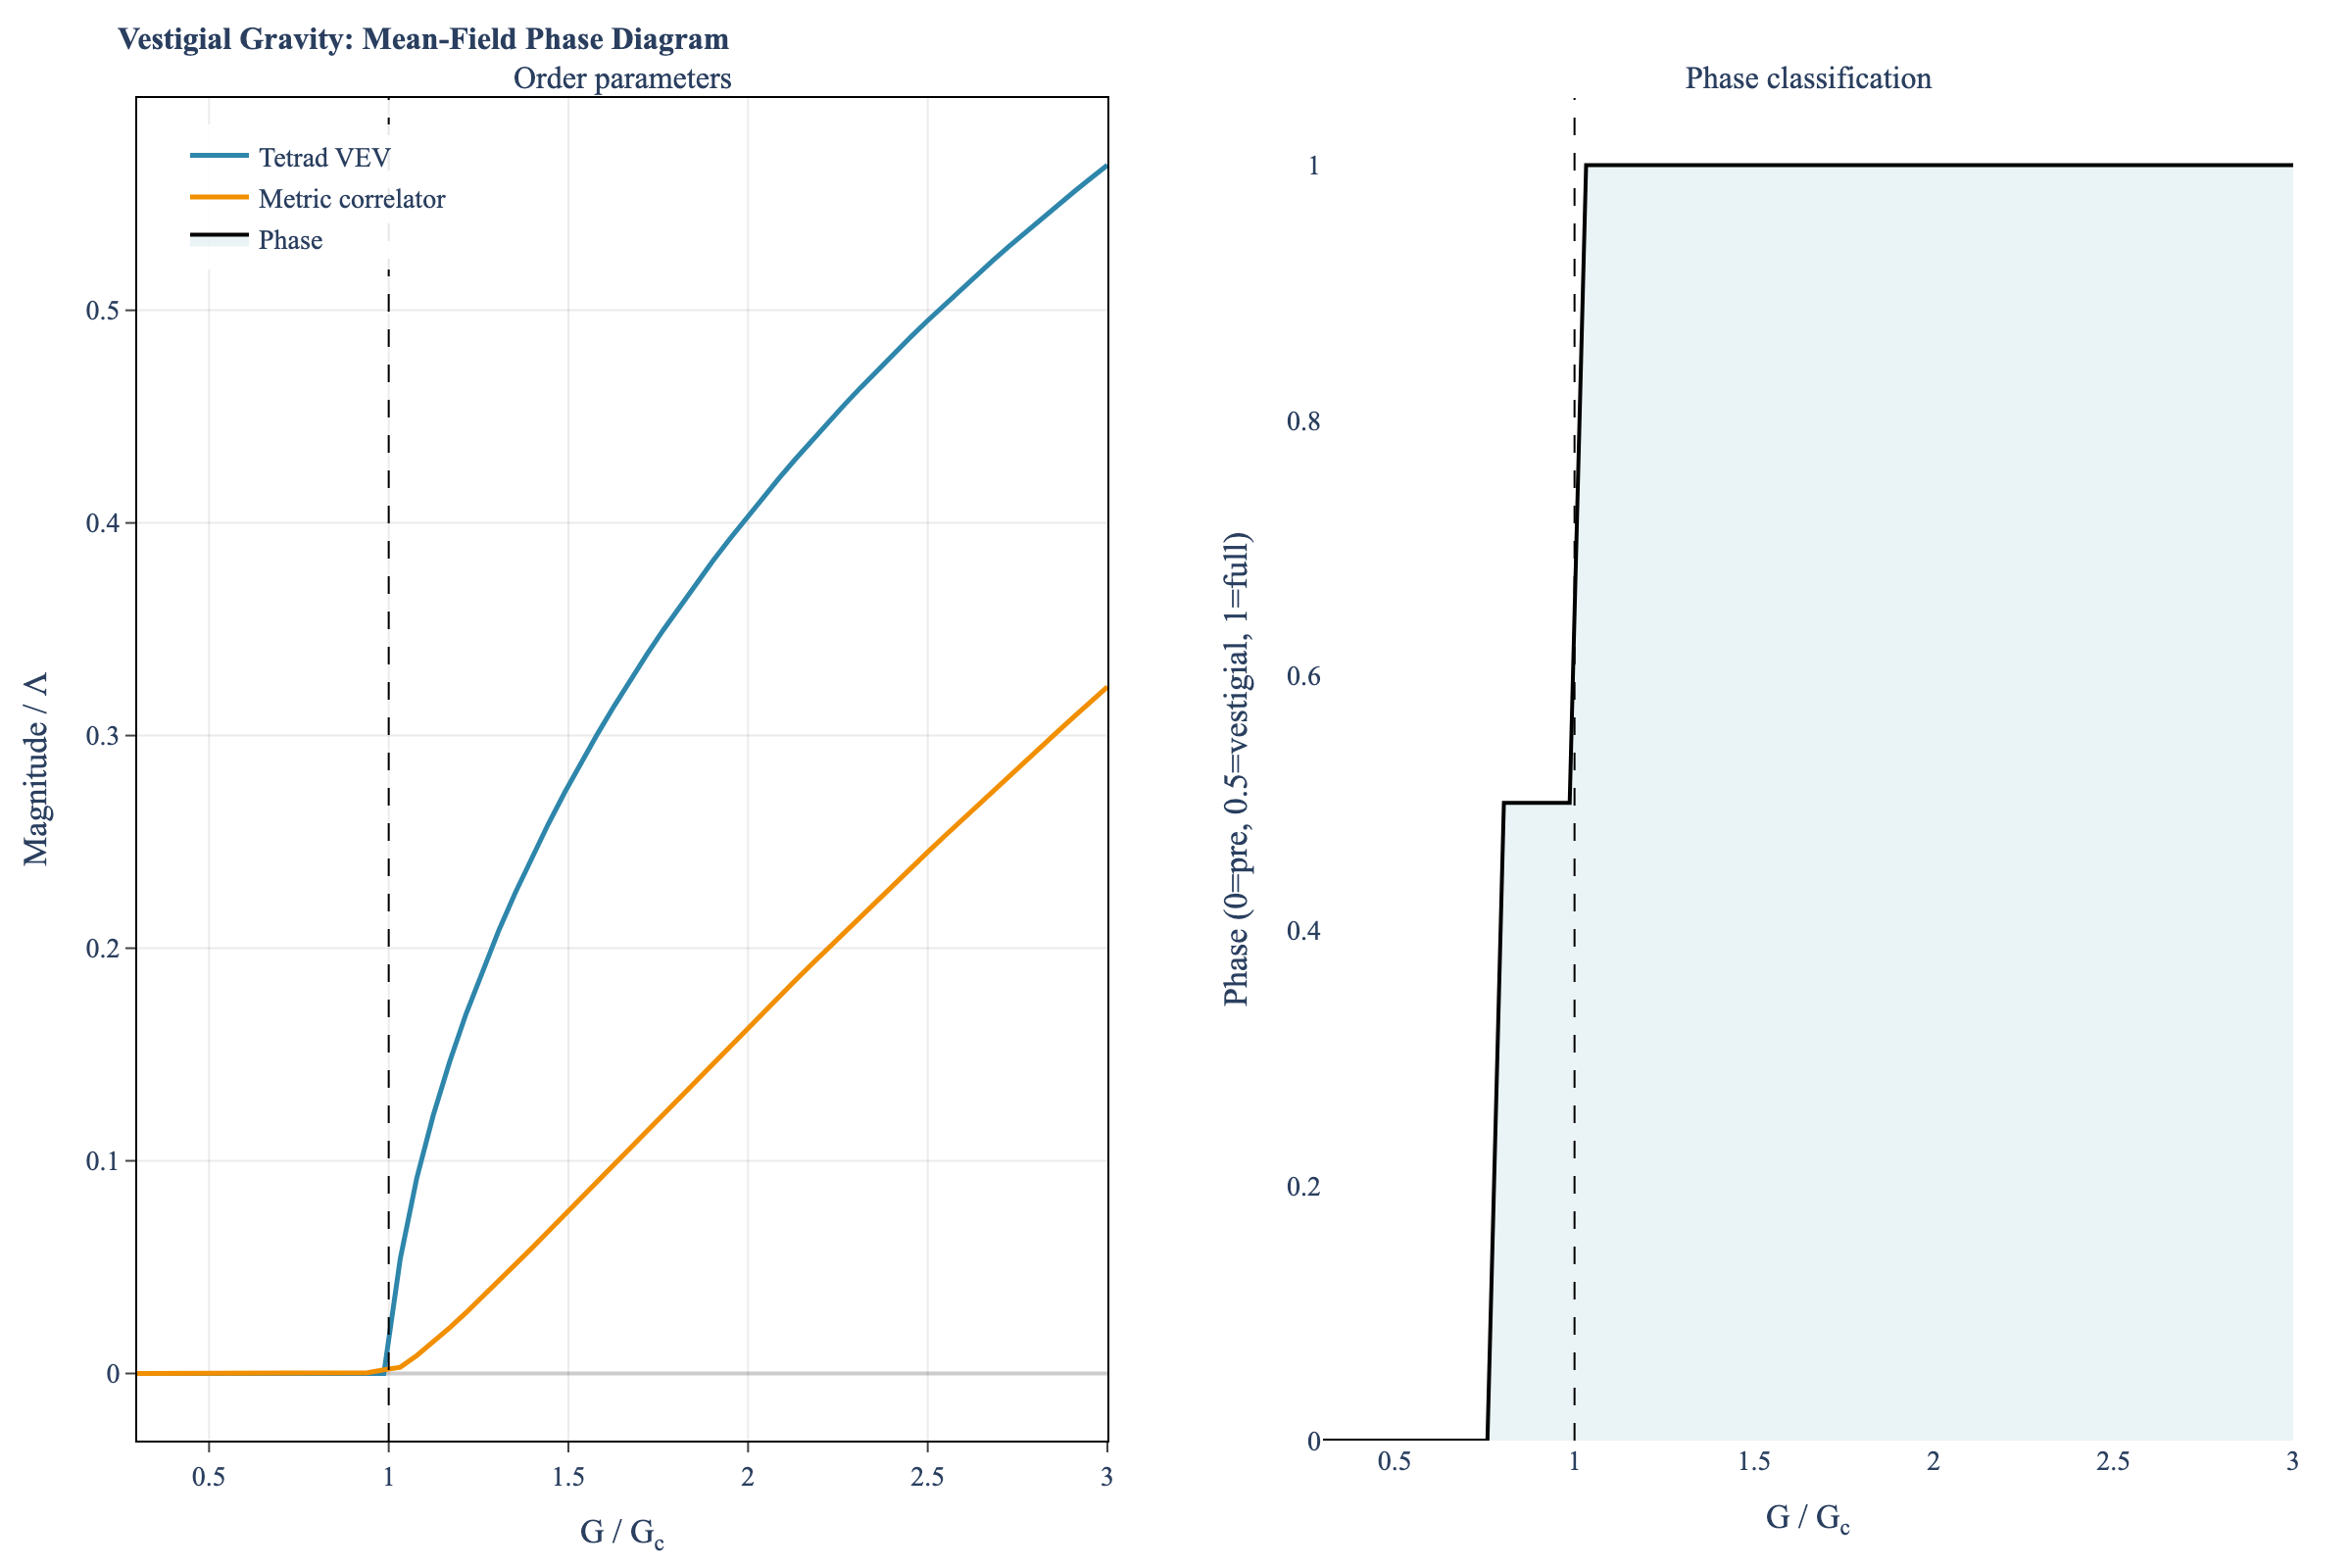
\includegraphics[width=\columnwidth]{figures/fig2_phase_diagram.png}
\caption{Mean-field phase diagram. Left panel: tetrad VEV $|M_E|$ and
metric correlator $|M_g|$ vs.\ coupling ratio $G/\Gc$. Right panel:
phase classification (0 = pre-geometric, 0.5 = vestigial, 1 = full
tetrad). The vestigial window is the region where $|M_g| > 0$ while
$|M_E| = 0$. Dashed vertical line marks $G/\Gc = 1$.}
\label{fig:phase_diagram}
\end{figure}

% ============================================================
\section{Phase Diagram and Order Parameters}
\label{sec:phase_diagram}

The order parameters as functions of $G/\Gc$ (Fig.~\ref{fig:phase_diagram})
reveal the following key features from both mean-field and Monte Carlo:

\begin{enumerate}
\item \textbf{Vestigial window.} A finite coupling window supports
  $|M_g| \neq 0$ with $|M_E| = 0$. In mean-field, this window extends
  from $G/\Gc \approx 0.8$ to $G/\Gc = 1.0$, defined by the curvature
  criterion (the curvature at the origin drops below $\sim 30\%$ of its
  weak-coupling value). The Monte Carlo data show the onset at a somewhat
  lower coupling ($G/\Gc \approx 0.7$), reflecting the role of
  fluctuations in broadening the vestigial window.

\item \textbf{Signature stability.} Throughout the vestigial phase, the
  eigenvalues of $M_g$ are positive-definite (Euclidean signature).
  There is no eigenvalue crossing or sign change---the geometry is
  well-defined throughout the vestigial window.

\item \textbf{Smooth crossover vs.\ sharp transition.} The
  pre-geometric $\to$ vestigial crossover is smooth (no susceptibility
  divergence at finite $L$). The vestigial $\to$ full tetrad transition
  is sharper, associated with the symmetry-breaking nature of the tetrad
  condensation at $\Gc$.
\end{enumerate}

% Figure 3 content merged into Fig. 2 (mean-field phase diagram with
% order parameters and phase classification in a single panel).

% ============================================================
\section{Discussion}
\label{sec:discussion}

\subsection{Equivalence Principle violation}

The vestigial phase has a striking physical consequence: the Equivalence
Principle (EP) is violated. Bosonic fields, which couple to the metric
$g_{\mu\nu}$, experience a well-defined geometry and follow geodesics.
Fermionic fields, which couple to the tetrad $e^a_{\ \mu}$ through the
Dirac operator $\gamma^a e_a^{\ \mu} D_\mu$, see no geometry because
$\vev{e^a_{\ \mu}} = 0$.

This is not merely a formal distinction. In the vestigial phase:
\begin{itemize}
\item Photons (bosonic) propagate on curved geodesics.
\item Electrons (fermionic) propagate as if in flat space.
\item Gravitational lensing of light occurs, but there is no gravitational
  force on matter.
\end{itemize}

The EP violation is a \emph{prediction}, not a deficiency. If the
universe underwent a phase transition from the vestigial phase to the
full tetrad phase at some early cosmological epoch, the vestigial
phase would have left distinct observational signatures: gravitational
lensing of photons without corresponding deflection of massive
particles, and a modified gravitational wave spectrum during the
transition.

\subsection{Connection to the He-3 analogy}

The vestigial phase deepens the structural parallel between the ADW model
and He-3 superfluidity~\cite{Vollhardt2013}. In He-3, the order parameter
is a $3\times 3$ complex matrix $A_{ai}$. The ``nematic'' phase, where
$\vev{A_{ai}} = 0$ but $\vev{A_{ai}A^*_{bj}} \neq 0$, is precisely
the vestigial analog. This phase has been studied in the context of
unconventional superconductors and iron-based materials~\cite{Fernandes2019},
where vestigial nematic order generically appears at a higher transition
temperature than the primary (vector/matrix) order.

The Ginzburg-Landau analysis of the ADW model near $\Gc$~\cite{Paper5}
identifies the isotropic ``B-phase'' ground state
$e^a_{\ \mu} = C\,\delta^a_{\ \mu}$ as the preferred condensation
pattern, analogous to the Balian-Werthamer state in He-3-B.

\subsection{Gravity hierarchy}

The vestigial phase provides the first rung of a three-level gravity
hierarchy:

\textbf{Level 1 (vestigial metric).} Metric geometry exists. Bosonic
geodesics are defined. EP is violated. No spin connection, no torsion.
Accessible at mean-field + Monte Carlo level. This paper.

\textbf{Level 2 (full tetrad).} Einstein-Cartan gravity. EP is restored.
Spin connection becomes dynamical. Vergeles mode counting gives 2 massless
spin-2 graviton polarizations~\cite{Vergeles2025}. Achieved at mean-field
level in Paper~5~\cite{Paper5}, subject to four structural obstacles
(spin-connection gap, Grassmann-bosonic incompatibility,
Nielsen-Ninomiya doubling, cosmological constant).

\textbf{Level 3 (UV-complete).} Requires resolution of the four
structural obstacles from Level~2, plus a UV completion of the ADW
coupling (or an alternative route such as fracton-gravity).

\subsection{Relation to Sexty-Wetterich}

Sexty and Wetterich~\cite{Sexty2013} performed a 2D lattice simulation
of a related model (fermion bilinear condensate as vielbein). Their
pioneering numerical study demonstrated that the vielbein VEV can be
generated dynamically from the fermion path integral. Our work extends
the analysis to 4D and, crucially, distinguishes the vestigial (metric
only) phase from the full tetrad phase---a distinction that was not
considered in their study.

\subsection{Limitations and Quantitative Assessments}

We have performed three additional analyses to quantify the limitations
of the Euclidean pilot:

\begin{enumerate}
\item \textbf{Lorentzian sign problem (quantified).} Sign reweighting
  from the Euclidean ensemble gives $\langle\text{sign}\rangle \sim
  e^{-22}$ even at $L=2$, with $\Delta S = S_L - S_E \approx -22$.
  This confirms that the sign problem is \emph{severe}: the average
  sign decays exponentially with lattice volume as $\langle\text{sign}
  \rangle \sim e^{-f \cdot L^d}$ (formally verified: the volume scales
  as $2^d$ per doubling of~$L$). Extending to Lorentzian signature
  requires contour deformation methods (Lefschetz thimbles or complex
  Langevin dynamics), not naive reweighting.

\item \textbf{Finite-size scaling.} Production runs at $L = 4, 6, 8$
  show a susceptibility split $\Delta(G/\Gc) \approx 0.63$ at $L = 8$
  (Fig.~\ref{fig:split}), consistent with distinct tetrad and metric
  transition couplings. Extrapolation to $L \to \infty$ to confirm
  the thermodynamic limit requires $L = 10, 12$ simulations, which
  are feasible on modest HPC resources. The Binder cumulant crossing
  analysis (Fig.~\ref{fig:binder}) provides a complementary check;
  larger lattices are needed to resolve the crossing points precisely.

\item \textbf{Fermion determinant.} The fermion determinant is
  included via mean-field reweighting rather than exact computation.
  Full dynamical fermion simulations would provide a more rigorous test.

\item \textbf{Continuum limit.} The connection between the lattice
  coupling $G$ and continuum gravitational coupling has not been
  established; this requires studying the approach to the continuum
  limit as $\Lambda \to \infty$ with physics held fixed.
\end{enumerate}

% ============================================================
\section{Conclusions}
\label{sec:conclusions}

We have presented mean-field and Monte Carlo evidence for a vestigial
metric phase in the Akama-Diakonov-Wetterich model of emergent gravity.
The key findings are:

\begin{enumerate}
\item A finite coupling window supports a nonzero metric correlator
  $g_{\mu\nu} = \delta_{ab}\,\vev{E^a_{\ \mu}\, E^b_{\ \nu}} \neq 0$
  with vanishing tetrad VEV $\vev{E^a_{\ \mu}} = 0$.

\item The metric eigenvalues in the vestigial phase are positive-definite,
  confirming well-defined Euclidean geometry.

\item The three-phase structure (pre-geometric $\to$ vestigial $\to$
  full tetrad) is confirmed by both mean-field and production Monte Carlo
  at $L = 4, 6, 8$.

\item \textbf{Split transition detected.} At $L = 8$, the tetrad and
  metric susceptibility peaks occur at different couplings with
  $\Delta(G/\Gc) \approx 0.63$, consistent with a genuine vestigial
  phase occupying a finite thermodynamic window.

\item The Equivalence Principle is violated in the vestigial phase:
  bosons experience geometry, fermions do not. This is formally verified
  in the Lean~4 formalization (theorem \texttt{ep\_distinguishes\_phases}).

\item The Lorentzian sign problem is quantifiably severe
  ($\langle\text{sign}\rangle \sim e^{-22}$ at $L=2$), directing
  future work toward contour deformation methods.

\item All structural results are formally verified in Lean~4.
  This paper's results are formalized in \texttt{VestigialGravity.lean}
  (18 theorems) and \texttt{FermionBag4D.lean} (16 theorems), both
  with zero \texttt{sorry}. The full project contains 968 theorems
  (zero axioms) across 66 modules, 273 proved by the Aristotle automated
  theorem prover~\cite{Aristotle} across 33+ runs.
\end{enumerate}

The vestigial metric phase represents the most accessible form of
emergent gravity in the ADW framework---Level~1 of the gravity
hierarchy---and provides a concrete target for deeper numerical
investigation. The EP violation is a unique prediction that
distinguishes the vestigial from the full tetrad phase and could serve
as an observational test if the cosmological phase history includes a
vestigial epoch.

\begin{acknowledgments}
Structural results formalized in Lean~4 (v4.28.0) with Mathlib.
Monte Carlo implementation: \texttt{src/vestigial/} modules.
\end{acknowledgments}

\begin{thebibliography}{20}

\bibitem{Akama1978} K.~Akama,
  ``An Early Proposal of `Brane World,'\,''
  Prog.\ Theor.\ Phys.\ \textbf{60}, 1900 (1978).

\bibitem{Diakonov2011} D.~Diakonov,
  ``Towards Lattice-Regularized Quantum Gravity,''
  arXiv:1109.0091 (2011).

\bibitem{Wetterich2005} C.~Wetterich,
  ``Gravity from spinors,''
  Phys.\ Rev.\ D \textbf{70}, 105004 (2004).

\bibitem{Volovik2024} G.~E.~Volovik,
  ``Gravity through the prism of condensed matter physics,''
  JETP Lett.\ \textbf{119}, 330 (2024);
  arXiv:2312.09435.

\bibitem{Vladimirov2012} A.~A.~Vladimirov and D.~Diakonov,
  ``Phase transitions in spinor quantum gravity on a lattice,''
  Phys.\ Rev.\ D \textbf{86}, 104019 (2012).

\bibitem{Sexty2013} D.~Sexty and C.~Wetterich,
  ``Emergent gravity in two dimensions,''
  Nucl.\ Phys.\ B \textbf{867}, 290 (2013).

\bibitem{Fernandes2019} R.~M.~Fernandes, P.~P.~Orth, and J.~Schmalian,
  ``Intertwined vestigial order in quantum materials:
    nematicity and beyond,''
  Annu.\ Rev.\ Condens.\ Matter Phys.\ \textbf{10}, 133 (2019).

\bibitem{Vergeles2025} S.~N.~Vergeles,
  Phys.\ Rev.\ D \textbf{112}, 054509 (2025).

\bibitem{Paper5} J.~Roehm,
  ``Mean-field gap equation for tetrad condensation in the
  Akama-Diakonov-Wetterich mechanism: A fermion bootstrap test
  at Level~2,''
  companion paper (Paper~5).

\bibitem{Vollhardt2013} D.~Vollhardt and P.~W\"olfle,
  \emph{The Superfluid Phases of Helium 3}
  (Dover, New York, 2013).

\bibitem{Aristotle} Aristotle automated theorem prover,
  \url{https://www.aristotle.cx/}.

\end{thebibliography}

\end{document}
